\documentclass[runningheads,a4paper]{llncs}

\usepackage[english]{babel}
\usepackage{ifpdf}
\usepackage{llncsdoc}
\usepackage{hyperref}
\usepackage{cite}
%\usepackage[cmex10]{amsmath}

\usepackage{array}
\usepackage{mdwmath}
%\usepackage{mdwtab}

\usepackage{fixltx2e}
\usepackage{stfloats}
\usepackage{float}
\usepackage{graphicx} % Required for the inclusion of images
\usepackage{amsmath} % Required for some math elements 
\usepackage{caption}

\usepackage{url}
\usepackage{algorithmic}
\usepackage{listings}

\usepackage{enumitem}
\usepackage{subfig}
\usepackage{comment}
\makeatletter

\usepackage{color}
\usepackage{amssymb}
\setcounter{tocdepth}{3}
\usepackage{graphicx}

\usepackage{fancyvrb}
\newcommand{\ygg@basicalert}[2]{\fbox{\bfseries\sffamily\scriptsize#1}{\sf\small$\blacktriangleright$\textit{#2}$\blacktriangleleft$}}
\newcommand{\annote}[2]{\ygg@basicalert{\textsc{#1}}{\textcolor{red}{#2}}}

%\newcommand{\annote}[2]{\ygg@basicalert{\textsc{#1}}{\textcolor{red}{#2}}}
\newcommand{\mohamed}[1]{\annote{Mohamed}{#1}}
\newcommand{\todomohamed}[1]{\annote{TODO-Mohamed}{#1}}

\newcommand{\katrina}[1]{\annote{Katerina}{#1}}
\newcommand{\todokatrina}[1]{\annote{TODO-Katerina}{#1}}
%
\newcommand{\heiko}[1]{\annote{Heiko}{#1}}
\newcommand{\todoheiko}[1]{\annote{TODO-Heiko}{#1}}

\lstset{
 % frame=top,frame=bottom,
  basicstyle=\small\normalfont\sffamily,    % the size of the fonts that are used for the code
  stepnumber=1,                           % the step between two line-numbers. If it is 1 each line will be numbered
  numbersep=10pt,                         % how far the line-numbers are from the code
  %tabsize=2,                              % tab size in blank spaces
  extendedchars=true,                     %
  breaklines=true,                        % sets automatic line breaking
  captionpos=b,                           % sets the caption-position 
  mathescape=true,
  %stringstyle=\color{white}\ttfamily, % Farbe der String
  %showspaces=false,           % Leerzeichen anzeigen ?
  %showtabs=false,             % Tabs anzeigen ?
  xleftmargin=6pt,
  framexleftmargin=3pt,
  framexrightmargin=3pt,
%  framexbottommargin=30pt,
%  framextopmargin=5pt,
%  showstringspaces=false      % Leerzeichen in Strings anzeigen ?
 }

\DeclareCaptionFormat{listing}{\rule{\dimexpr\textwidth+17pt\relax}{0.4pt}\par\vskip1pt#1#2#3}
%\captionsetup[lstlisting]{format=listing,singlelinecheck=false, margin=7pt, font={sf}}%,labelsep=space}%,labelfont=bf}

%\renewcommand\lstlistingname{Algorithm}

\DeclareMathVersion{sans}
\SetSymbolFont{operators}{sans}{OT1}{cmbr}{m}{n}
\SetSymbolFont{letters}  {sans}{OML}{cmbrm}{m}{it}
\SetSymbolFont{symbols}  {sans}{OMS}{cmbrs}{m}{n}

\lstnewenvironment{sflisting}[1][]
  {\lstset{#1}\mathversion{sans}}{}
  
%\usepackage{caption}
%\captionsetup[figure]{font=small,skip=0pt}   

\begin{document}
\section{Introduction}\label{sec:introduction}

rSLA is a domain specific language (DSL) for expressing and managing service level agreements (SLAs) in a cloud environment. rSLA is coded in Ruby \cite{ruby}, a dynamic language that enables rapid prototyping and application development. 

The rSLA DSL is described by an alphabet and by production rules that help to extend the language. The rSLA programming library provides a runtime engine for deploying and running an rSLA service in a cloud environment.

Although the scientific literature provides plentiful results on automated management of SLAs for distributed computing \cite{wsla, wsag}, cloud markets hesitate to adopt such solutions. Provisioning of cloud services is handled either manually or with software tools that do not embrace cloud service characteristics.

Cloud service management does not yet support automated and transparent solutions for the management of leased resources. Additionally, there is no established standard yet for the automatic expression and management of SLAs for cloud services.

rSLA provides a DSL library for the definition of rSLA objects and a runtime engine to create and process such objects. The DSL enables the automated generation of customized SLAs and the transparent management of cloud service compliance.

The rSLA is deployed on the IBM Bluemix platform \cite{bluemix} as a ruby web service using the sinatra gem\footnote{Sinatra, \url{http://www.sinatrarb.com/}}. A pilot version of the language is currently running for an IBM financial client. The monthly results from using the rSLA language to evaluate the service level compliance of resources leased by the client, showcase the rSLA DSL adequacy in managing cloud services.

How is the paper structured

-what is the problem that the language solves, motivation to solve this problem
-language structure, alphabet, production rules
-language runtime
-current testing, future testing

\section{Problem definition/ motivation}
\label{sec:problem}
Cloud service management does not yet support enough automated and transparent solutions for the management of leased resources. 

There is no established standard so far for the automatic expression and management of SLAs for cloud services.

The rSLA language is not intended to be used only by engineers. An important goal in the language design is to provide a high-level, easy to use and 
to extend tool that is suitable either for human or machine consumption.


\section{rSLA DSL}
\label{sec:dsl}
alphabet, vocabulary, language structure

production rules


\subsection{rSLA language structure, alphabet}

 point of this subsection?

The rSLA language follows the semantic decomposition of the WSLA specification \cite{wsla}, where an SLA takes the form of a hierarchical tree with a 
single root node and numerous uni-directional edges. Figure \ref{rSLA_diag} illustrates the rSLA vocabulary as a tree of classes that the rSLA DSL 
implements. Connections between nodes in the rSLA tree highlight the nesting of SLA context. 

In the rSLA alphabet the root node of an rSLA tree represents an SLA object. In Figure \ref{rSLA_diag} nodes that are positioned close to the root, 
designate branches of SLA context (e.g. base and composite metrics, service level objectives). Edges between nodes are uni-directed to illustrate the 
rSLA tree hierarchical schema.

\begin{figure}
  \centering
    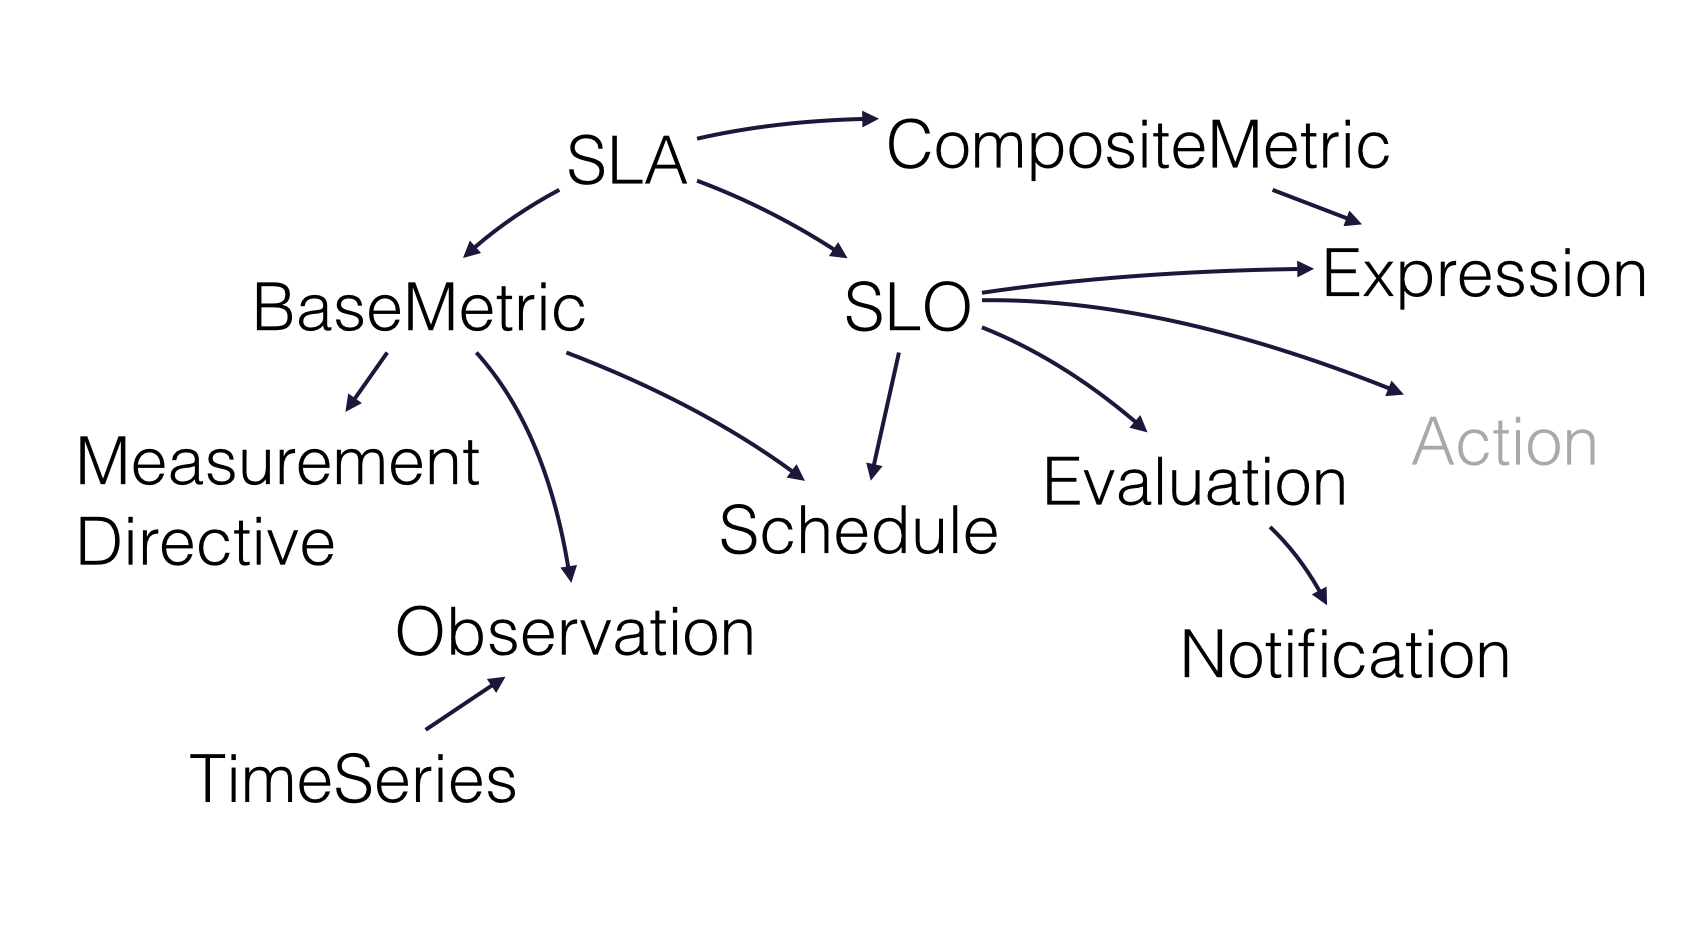
\includegraphics[width=0.5\textwidth]{pics/rslauser}
    \caption{rSLA DSL class diagram}
    \label{rSLA_diag}
\end{figure}

 rSLA supports the creation of programming blocks that express SLA context and that are necessary to run and manage rSLAs in a cloud environment. 
Listing \ref{lst} describes the rSLA vocabulary using set notation to highlight the nesting between language objects:
\begin{lstlisting}[breaklines, mathescape, firstnumber=auto, caption=rSLA vocabulary, label=lst]
SLA $\supset$ { BaseMetric+, CompositeMetric*, SLO+ }
BaseMetric $\supset$ { MeasurementDirective, Observation*, Schedule* }
CompositeMetric $\supset$ { Expression* }
SLO $\supset$ { Expression*, Action*, Evaluation*, Schedule* }
\end{lstlisting}

In the rSLA language nested relationships denote inclusive associations between objects. For example, an SLA includes base and composite metrics as 
well as SLOs. Inclusive relationships of rSLA objects do not share same multiplicity rules (listing \ref{lst}). The rSLA DSL follows the WSLA 
specification \cite{wsla} with respect to the definition of rSLA objects and of their basic attributes.

In Figure \ref{rSLA_diag} the $Notification$ and $TimeSeries$ classes do not appear in the rSLA set representation. These two classes produce objects 
that help with service level management operations like the statistical analysis of data coming from monitoring or automated notification reports on 
scheduled events of service level evaluation. Such two classes are not initially required to build and run SLA instances in a cloud environment, but 
may be required while one or more SLA management tasks are processed.



conclude that
 
\subsection{rSLA language production rules}

rSLA language constructs: elements have relationships/dependencies, there is nesting and management dependencies

production rules

\section{rSLA runtime engine}\label{runtime}

The rSLA is implemented as a DSL for cloud SLAs. The rSLA programming library, currently, provides support for the following SLA management operations that take place while a provisioned service is running:
\begin{enumerate}
\item SLA creation and activation.
\item monitoring and measurement of service metrics as specified by the SLA context.
\item storage and processing of observed service metric values and of SLO evaluation results. 
\item scheduling of rSLA objects.
\item service level evaluation.
\item notification events: reports.
\end{enumerate}
The next paragraphs highlight rSLA implementation aspects for all supported operations.

\subsection{SLA creation and activation}

As discussed in Chapter \ref{dsl}, rSLA editing takes place using ruby programming blocks. The rSLA language takes advantage of this Ruby coding feature and exposes rSLA objects through multi-lined do..end coding blocks. When an rSLA runtime engine reads a new rSLA block, it generates a new rSLA object that belongs to the block related class. The attributes and function behavior of the generated object are mapped from the ruby block context. 

Listing \ref{basescript} describes an rSLA script for the creation of an SLA and of a base metric. The script can run in an rSLA service runtime environment to generate the two respective objects and to activate a schedule for the value measurement of the base metric.

\begin{minipage}{0.9\textwidth}
\begin{lstlisting}[language=Ruby, basicstyle=\small\normalfont\sffamily, breaklines=true,  captionpos=b, mathescape=true, caption=rSLA SLA (lines 1-4) and basemetric (lines 6-19) creation script, label=basescript, numbers=left, numbersep=5pt, numberstyle=\tiny] 
sla do
  tenant "Demo"
  provider "IBM"
end  

basemetric do
    name "bareMetalProvisioning"
    unit "provisioningtime"
    measurementdirective do
    	entity "baremetal"
    	type "jsonArray"
    	source "http://provisioningxlet.stage1.mybluemix.net/server/baremetal/provisioningtime" 
  	end
  schedule do    
  	frequency "1"
    unit "m"
    method "every"
  end
end
\end{lstlisting}
\end{minipage} 

The block for the creation of the SLA object simply describes two strings that designate the names of the SLA tenant and provider. The rSLA engine reads such strings as the attribute values of the newly created SLA object. Similarly, the rSLA interpreter reads the base metric block and create a new base metric object that inherits the attributes of the rSLA BaseMetric class. 

In the base metric block, a DSL user can define BaseMetric object attributes like the base metric name and measurement unit. Additionally, a DSL user can specify directives for the measurement of the created metric. A measurement directive represents a concept that is inherited from the WSLA specification \cite{wsla}. 

The rSLA DSL exposes a measurement directive as a block of statements that a DSL user can specify. Such statements describe the configuration of a measurement directive object that guides the value measurement of the parent base metric. A measurement directive indicates the result type that is expected from a base metric measurement.

In the measurement directive block, the term entity is used for the representation of restful \footnote{ReST: \url{http://en.wikipedia.org/wiki/Representational_state_transfer}} endpoints. Such may have a URL\footnote{Unique Resource Locator: \url{http://en.wikipedia.org/wiki/Uniform_resource_locator}} form: \url{http://provisioningxlet.stage1.mybluemix.net/server/baremetal/provisioningtime}. A measurement directive object uses an attribute named $source$ to denote the restful endpoint for fetching the relevant base metric value. The rSLA MeasurementDirective class provides an example on how to define measurement directive objects for rSLA base metrics. Such example, like the illustrated block of Listing \ref{basescript} can be extended accordingly. 

Last but not least, a DSL user can specify the details of a schedule for the measurement of the base metric. The schedule block details are explained in Section \ref{schedule}.

\subsection{monitoring and measurement}
Any SLA management framework for cloud services needs a tool for monitoring and measuring service metric values. In a cloud runtime environment, an rSLA service currently uses Java Xlets \cite{xlets} to handle the monitoring of base betric values. Chapter \ref{deployment} describes in detail the configuration and functionality of Xlets with the deployment of rSLA as a compliance service in a cloud environment.

In an rSLA service, monitoring and measurement operations are controlled by one or more schedules. Every base metric follows its own schedule. Measured metric values are collected to a backend database for further processing. 
\subsection{storage and processing}
Observed values of base metrics are stored during service provisioning. These data values are required for the computation of composite metric values, which in turn are used in the service level evaluation. 

Currently, rSLA has been deployed using the Cloudant document database \cite{cloudant}. The values of base metrics are preserved as observation documents that also keep a timestamp on the measurement time and the associated base metric id. Cloudant uses map and reduce statements to collect and to efficiently process data values. 

rSLA uses CouchRest \cite{couchrest} to access Cloudant using HTTP requests and the CouchRest model to map rSLA object properties in the data middleware. Associations between rSLA objects are, at the present time, described through the rSLA Cloudant data schema. Figure \ref{schema} illustrates currently supported associations between rSLA objects.

Base, composite metrics as well as SLOs are associated with an SLA instance by a $belongs_to$ relationship. Similarly, a set of observations $belongs_to$ a base metric and a set of evaluation and notification data to an SLO. 

The $belongs_to$ feature is defined in the CouchRest model as a property for the association of documents. It resembles a $has-a$ composition relationship where a constituent object belongs to or is part of another object. In an rSLA cloudant environment 


\begin{figure}
\centering
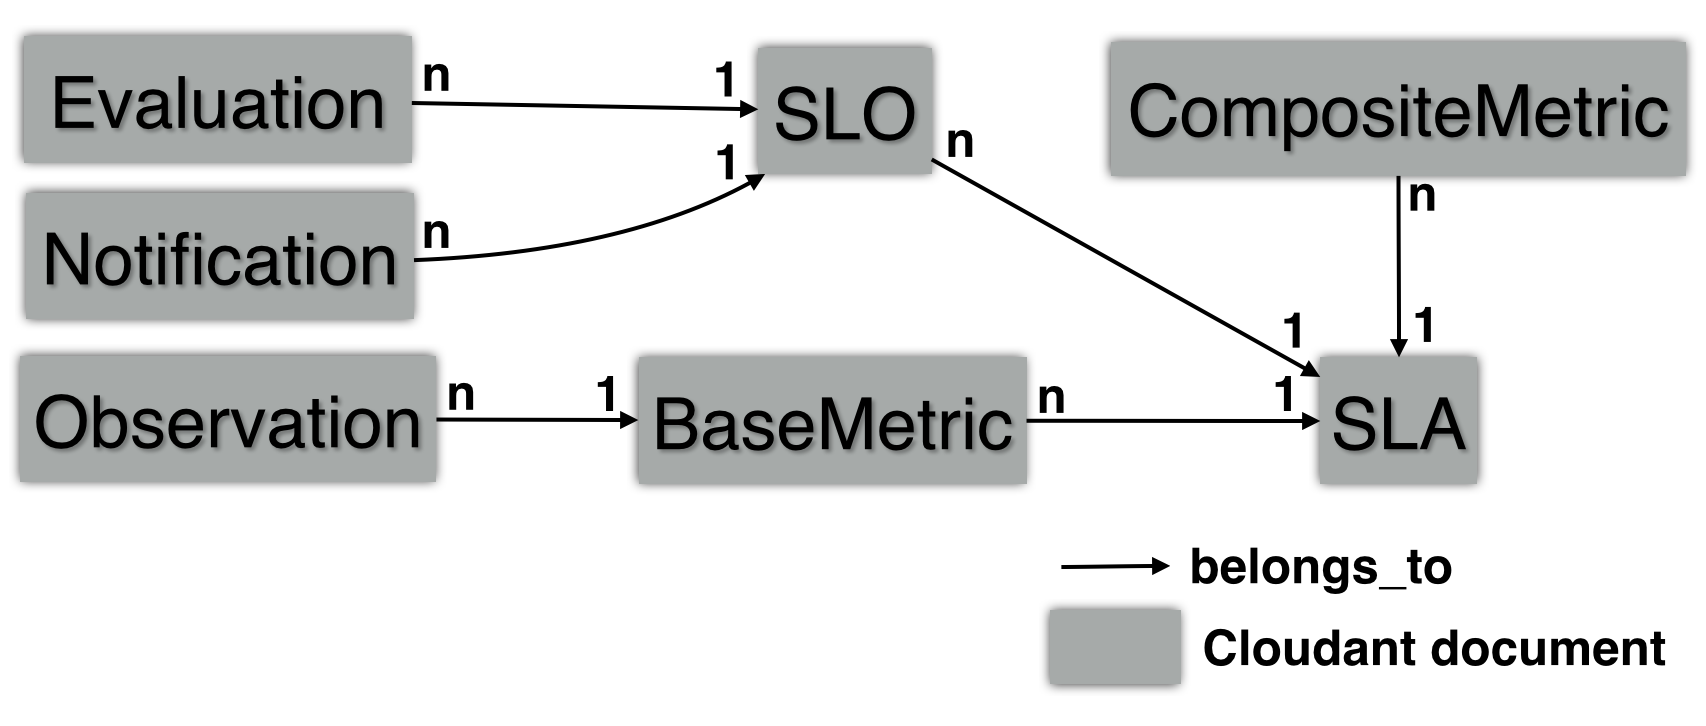
\includegraphics[width=0.8\textwidth]{pics/schema}
\caption{\label{schema} rSLA Cloudant object associations}
\end{figure}


Processing, at the current implementation state, refers to compositions of service value sets for the creation of new rSLA objects.

timeseries: ready to use functions
\subsection{scheduling}\label{schedule}
The rSLA BaseMetric class provides methods for configuring a base metric object with one or more schedules.
\subsection{service level evaluation}

\subsection{notification reports}
can also be alerts
rSLA needs a source for monitoring data and a tool for reporting.

\section{rSLA deployment }

rSLA Service has literally been evolved on the IBM Bluemix PaaS as a ruby Sinatra application. As shown in Figure~\ref{fig:runtime}, the different components involved in SLA 
management are deployed in Bluemix. The following section will explain further how rSLA interoperates with the other services (Scheduler, Cloudant, Xlets) in a real use case. 

\begin{figure}[H]
\centering
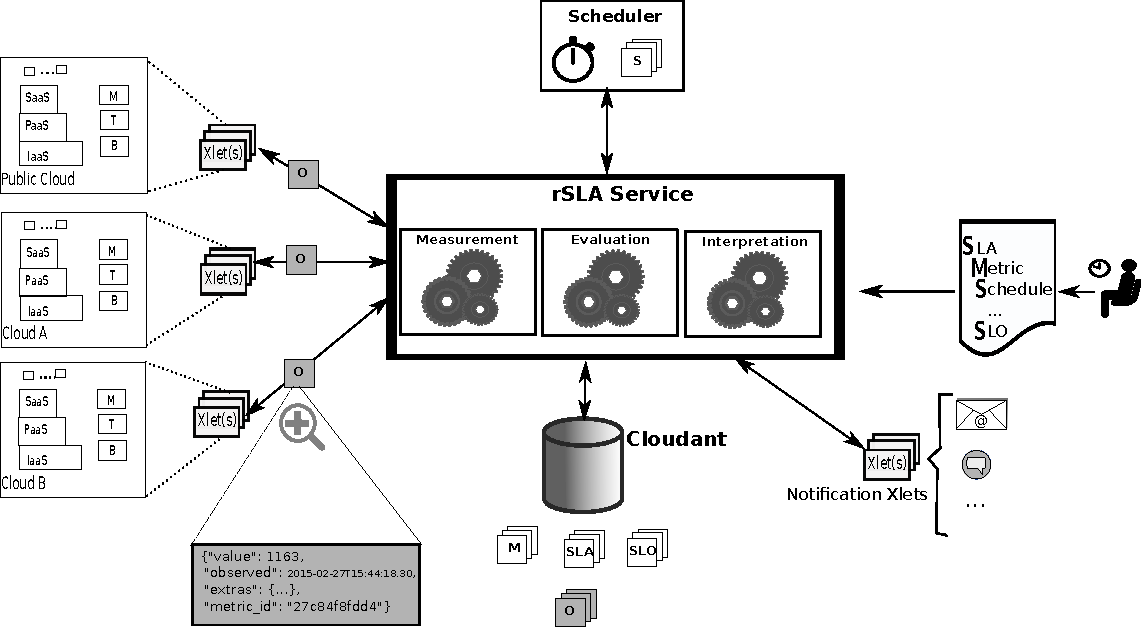
\includegraphics[width=\textwidth]{pics/runtime.pdf}
\caption{\label{fig:runtime} rSLA runtime}
\end{figure}


\subsection{Ameriprise pilot}

Currently, the rSLA service supports the management of cloud services that are leased by an existing customer. In one agreement, the IBM customer migrated a workload from a customer-owned, on-premise data center environment to the IBM cloud.  Along with the move, the customer required the monitoring of seven custom SLAs that had never been offered previously by the service provider in the cloud.

Each of the seven running SLAs consist of one base metric and one service level objective. The rSLA service that is running on the Bluemix platform, is aware of these seven agreements' context as such information is parsed by the rSLA engine to activate and initiate the measurement of involved base metrics. The rSLA service monitors, measures, evaluates and reports the service level status of the seven involved SLOs on a daily basis to the customer. 

%can we add a graph showing statistics on the rSLA service usage/performance since we started the ameriprise pilot? Bluemix?
%or from cloudant?



\subsection{rSLA service}
rSLA Service is a Sinatra application deployed on Bluemix PaaS. It offers different REST interfaces that allow the management of the life cycle of an SLA described using our DSL.
At the reception of a new SLA, rSLA Service interprets the file and creates ruby objects based on the DSL. The new objects are persisted in Cloudant using CouchRest Model.
On the activation of an SLA, rSLA Service orchestrates all the needed operations to activate and manage the SLA life cycle. It starts by scheduling data collection for base 
metrics. As shown in Figure~\ref{fig:runtime}, based on the defined schedules, the scheduler triggers the needed rSLA Service interfaces. This latter will then invoke the 
Monitoring Xlets to collect new observations for the related base metrics. Afterwards, the observations are persisted in Cloudant. Similarly, on the schedule of an SLO, the 
Scheduler triggers a rSLA Service interface for SLO evaluation. rSLA will then evaluate the data related to the specific SLO. This evaluation implies 
eventually the usage of map-reduce functions offered by Cloudant. We made this decision in order to delegate all the possible parallel processings to Cloudant and benefit from its 
efficiency. Afterwards, rSLA Service generates JSON notifications representing the results of the evaluation. These notifications are sent to the Notification Xlet for 
formatting and reporting to the client.   
\subsection{rSLA Xlets}
During its life-cycle, rSLA Service requires different services to ensure the management of SLAs. These services are eventually offered as services through Bluemix PaaS. At the 
time being, rSLA uses one offered service for persistence and a list of services for monitoring and reporting. These latter, are provided as Xlets. An Xlet is a light weight 
application offered as a service through Bluemix PaaS. This application is designed to facilitate the integration of different offered services spanning over the different layers 
of the Cloud by providing a generic REST API. An Xlet is customized according to its role in the overall system. As shown in Figure~\ref{fig:xlet}, each Xlet provides three 
interfaces:
\begin{itemize}
 \item \emph{CFBrokerInterface}: Since the Xlets are provided as services by Bluemix PaaS, they need to offer this generic interface that describes exactly how to provision the 
service, how to unprovision it, how to bind the service to a given application and how to unbind it. 
\item  \emph{ConfigurationInterface}: In order to ensure multi-tenancy and customization of an Xlet, it should offer an interface to configure its tenancy. This interface could 
offer other functionalities of customization. It allows in some cases to configure the access credentials for Cloud resources.
\item  \emph{RuntimeInterface}: This interface describes the main business of the Xlet. It describes the specific functionalities to be offered by the application instance (e.g., 
monitoring services, reporting services). 
\end{itemize}
\begin{figure}[H]
\centering
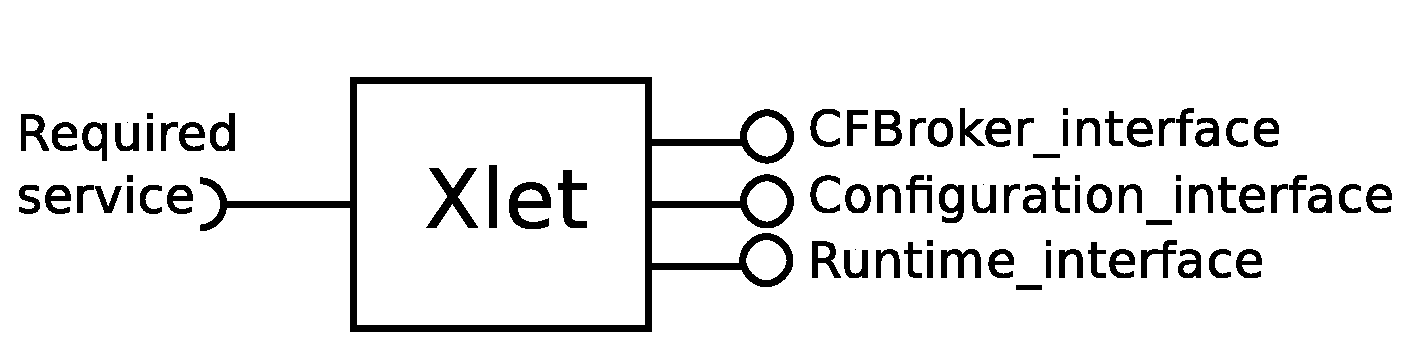
\includegraphics[width=0.6\textwidth]{pics/Xlet}
\caption{\label{fig:xlet} Xlet generic design}
\end{figure}

All Xlets respect the same architecture but differs in their implementations from a use case to another. In our current work we defined different monitoring and reporting Xlets. 
Monitoring Xlets are in-line with the DMTF standard. They allow collecting monitoring data for a specific type of resources with different granularities. For example, 
Figure~\ref{fig:slxlet} shows a SoftLayer specific Xlet. SLXlet allow to get monitoring data of SoftLayer provisioned servers for a given account. The account credentials are 
passed to the Xlet in the configuration phase through the Configuration interface. Afterwards, the Runtime interface of the Xlet could be used to get the list of servers, the list 
of metrics for a given server or, the value for a given metric for a specific server.

\begin{figure}[H]
\centering
\hspace{1.5cm}
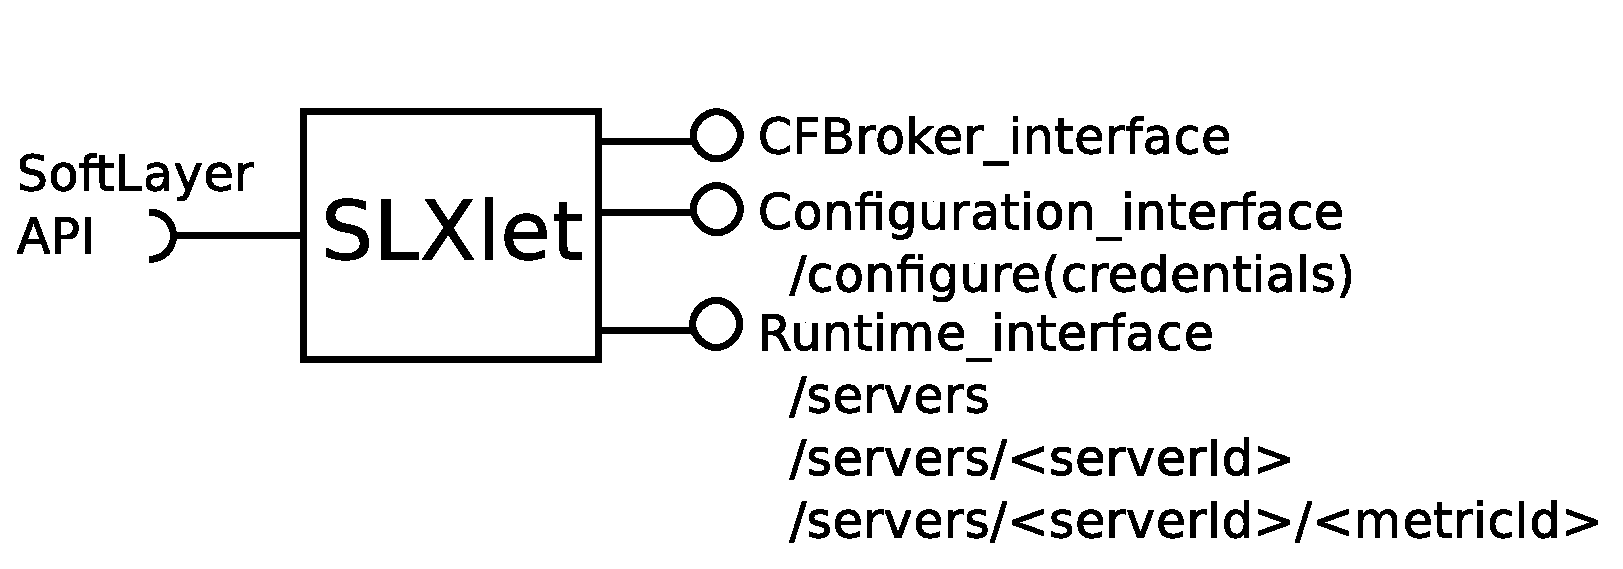
\includegraphics[width=0.7\textwidth]{pics/SLXlet}
\caption{\label{fig:slxlet} SoftLayer Xlet design}
\end{figure}

Using Xlets within Bluemix PaaS has been very helpful. The advantageous characteristics of using Xlets in this environment are the following:
\begin{itemize}
 \item Scalability: this characteristic is inherited from the scalability of Bluemix environment. Since the Xlet could be provisioned as an application or a service within 
Bluemix, it is easy to scale it horizontally to cope with the work load by adding or removing new instances,
\item Reusability: all Xlets have a common and generic core code that allow the easy reusability with minor modifications for specific use case, 
\item Manageability: managing Xlets is handled to Bluemix, the management here includes provisioning, deprovisioning, binding and unbinding Xlets to other applications,
\item Flexibility: Xlets could be integrated easily using Bluemix services, they could be provisioned using different plans (e.g., shared or dedicated). 
\end{itemize}

\bibliographystyle{splncs}

\bibliography{mainDoc}

%----------------------------------------------------------------------------------------


\end{document}
